\documentclass[conference]{IEEEtran}
\IEEEoverridecommandlockouts
\usepackage{amsmath,amssymb,amsfonts}
\usepackage{bm}
\usepackage{booktabs}
\usepackage{graphicx}
\usepackage{microtype}
\usepackage{xcolor}
\usepackage[hidelinks]{hyperref}
\setlength{\textfloatsep}{4pt plus 1pt minus 1pt}

\newcommand{\bF}{\bm{F}}
\newcommand{\bG}{\bm{G}}
\newcommand{\bz}{\bm{z}}
\newcommand{\btheta}{\bm{\theta}}
\newcommand{\bpsi}{\bm{\psi}}
\newcommand{\bu}{\bm{u}}
\newcommand{\bd}{\bm{d}}
\newcommand{\ba}{\bm{a}}
\newcommand{\bb}{\bm{b}}
\newcommand{\bH}{\bm{H}}
\newcommand{\bA}{\bm{A}}
\newcommand{\bS}{\bm{S}}
\newcommand{\bW}{\bm{W}}
\newcommand{\cS}{\mathcal{S}}
\newcommand{\cA}{\mathcal{A}}
\newcommand{\cB}{\mathcal{B}}
\newcommand{\E}{\mathbb{E}}
\newcommand{\norm}[1]{\left\lVert #1\right\rVert}
\ifdefined\cameraready
\newcommand{\widefigwidth}{0.78\textwidth}
\else
\newcommand{\widefigwidth}{0.98\textwidth}
\fi
\newtheorem{assumption}{Assumption}
\newtheorem{proposition}{Proposition}
\newtheorem{theorem}{Theorem}
\newtheorem{corollary}{Corollary}

\title{Lyapunov-Controlled Minimax Policy Learning for Adversarial Dynamic Spectrum Access}

\author{
\IEEEauthorblockN{Jialin Zhuang and Vincent K. N. Lau}
\ifdefined\cameraready
\IEEEauthorblockA{Department of Electronic and Computer Engineering, The Hong Kong University of Science and Technology\\
Hong Kong SAR, China; Emails: jzhuangag@connect.ust.hk; eeknlau@ece.ust.hk}
\thanks{This work was supported by the Research Grants Council (RGC), Hong Kong, under the Areas of Excellence Scheme Grant AoE/E-101/23-N and AoE/E-601/22-R.
(Corresponding author: Vincent K. N. Lau.)}
\else
\IEEEauthorblockA{Department of Electronic and Computer Engineering\\
The Hong Kong University of Science and Technology, Hong Kong SAR, China}
\fi
}

\begin{document}
\maketitle

\begin{abstract}
Adaptive jamming makes dynamic spectrum access (DSA) a sequential zero-sum Markov game: both channel selections change packet service and hence the future queue state.
We propose Lyapunov-Controlled Minimax Policy Learning (LCMPL) for this queue-aware game.
LCMPL combines the simultaneous policy-gradient field with a Jacobian--field correction, gives the two directions separate step sizes, and regulates them using local game geometry and a communication-aware Lyapunov merit.
A curvature identity characterizes when the correction dissipates rotational saddle-field energy.
Under local smoothness, geometric coverage, and bounded learning and local-model errors, the time-averaged expected stationarity residual has an $O(1/K)$ transient plus an explicit residual term over $K$ joint updates.
A local policy-gap condition further converts this result into a bound on the transmitter's worst-case queue-aware utility loss.
Experiments show improved worst-case utility and exploitability over representative minimax learners; load sweeps further show that selective curvature control yields higher goodput and lower backlog near capacity.
\end{abstract}

\begin{IEEEkeywords}
Anti-jamming communications, dynamic spectrum access, reinforcement learning, minimax policy learning, zero-sum Markov games.
\end{IEEEkeywords}

\section{Introduction}
In dynamic spectrum access (DSA), a secondary transmitter selects a channel under incumbent activity and time-varying propagation \cite{Zhao2008Myopic}; practical access decisions must also account for switching delay, traffic backlog, interference, and jamming \cite{Celik2012DynamicServer,Naparstek2019DeepDSA,Liu2018SpectrumWaterfall,Wang2020AntiJammingSurvey}.
Adaptive jamming couples radio variation with opponent adaptation.
More importantly, a poor joint channel choice can prevent packet service, enlarge the queue, and change the next decision state.
The learning problem is therefore not a sequence of disconnected static games: its optimization dynamics directly affect future communication congestion.

\begin{figure}[t]
\centering
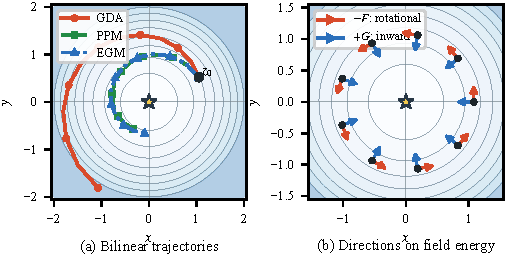
\includegraphics[width=0.64\columnwidth]{figures/mathematical_motivation.pdf}
\caption{Why saddle-field step sizes must adapt to local coupling.
For $\bz_{k+1}=\bz_k-\beta\bF_\omega+\gamma\nabla\bF_\omega\bF_\omega$, $\omega$ is coupling strength and $q_k=\|\bz_{k+1}\|/\|\bz_k\|$ is the one-step norm ratio.
(a)--(b) show rotation and correction; (c) shows that $q_k<1$ and the minimizing $\gamma/\beta$ vary with $\omega$; (d) shows a fixed ratio becoming expansive while the local ratio remains contractive.}
\label{fig:motivation}
\end{figure}

A two-player zero-sum Markov game captures this interaction \cite{Shapley1953StochasticGames,Littman1994MarkovGames}.
The transmitter policy $\pi_{\btheta}$ maximizes a discounted utility that rewards delivered packets and penalizes backlog, packet loss, and channel switching, while the jammer policy $\nu_{\bpsi}$ minimizes it.
Because their channel actions determine the service distribution, both players affect the queue transition as well as the immediate utility.
Their simultaneous policy gradients consequently form a coupled saddle field rather than a single improvement direction.

The main learning difficulty is rotational coupling.
As Fig.~\ref{fig:motivation} shows, gradient descent--ascent (GDA) can cycle in a bilinear local model, whereas the Jacobian--field action supplies radial contraction \cite{Balduzzi2018Mechanics}.
The useful balance changes with local coupling, so a fixed curvature-to-field step-size ratio can move from contraction to expansion as queue occupancy, radio conditions, and policies evolve.

The proximal point method (PPM) and extragradient method (EGM) suppress rotation by evaluating an implicit or extrapolated field \cite{Rockafellar1976PPM,Korpelevich1976Extragradient}.
Their local expansions share a Jacobian--field correction but couple its effective scale to the field step through a single step size \cite{Lu2022ODE}.
Adaptive Mirror-Prox methods tune extragradient updates from observed operator geometry \cite{Antonakopoulos2021AdaProx}, and double-step extragradient separates the extrapolation and update stages \cite{Hsieh2020DSEG}.
These methods establish the value of adaptive scaling; the remaining design question is how to balance the field and curvature coordinates as radio conditions and policies change.
Field-energy reduction alone can also favor a low-utility stationary policy, so it is not a sufficient criterion by itself.

In this paper, we propose Lyapunov-Controlled Minimax Policy Learning (LCMPL).
Following Lyapunov-drift step-size control \cite{Yuan2025StepSizeSDE}, LCMPL assigns separate step sizes to the field and Jacobian--field directions and selects them through a two-variable quadratic program (QP) that predicts local merit decrease.
The merit connects policy stationarity with worst-case queue-aware communication utility, while a same-state utility test rejects detrimental curvature.
We establish an $O(1/K)$ stationarity transient with an explicit learning-error residual and, under a local policy-gap condition, a worst-case utility bound.
Queue-aware experiments compare LCMPL with representative simultaneous-gradient, extragradient, implicit-update, and clipped-policy baselines and examine how the gain changes from light to near-capacity traffic.

\section{Adversarial DSA System and Markov-Game Model}
\subsection{Queue-Aware Wireless Interaction}
\begin{figure}[t]
\centering
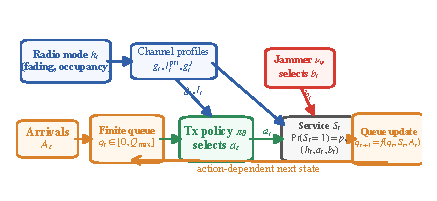
\includegraphics[width=0.98\columnwidth]{figures/system_model_queue.pdf}
\caption{Queue-aware adversarial DSA: both channel actions change packet service and the next queue state.}
\label{fig:system}
\end{figure}

Fig.~\ref{fig:system} considers a secondary transmitter with a finite buffer, its receiver, incumbent activity, and an adaptive jammer over $M$ subchannels.
At slot $t$, an exogenous mode $h_t\in\mathcal H=\{1,\ldots,L\}$ selects a correlated radio profile $x_t=(g_t,I_t^{\rm pri},g_t^J)$: secondary-link gains, incumbent interference, and jammer--receiver gains across channels.
The transmitter and jammer simultaneously choose $a_t\in\cA$ and $b_t\in\cB$, where $\cA=\cB=\{0,\ldots,M-1\}$.
The state
\[
s_t=(h_t,x_t,q_t,a_{t-1})\in\cS
\]
also contains queue length $q_t\in\{0,\ldots,Q_{\max}\}$ and the previous transmitter channel $a_{t-1}$.
Thus $h_t$ describes the external radio regime, while $q_t$ records the endogenous consequence of earlier joint actions.

Let $P_{\rm s}$, $P_{\rm J}$, and $N_0$ denote transmission power, jamming power, and receiver noise, respectively.
The factor $\ell(a,b)$ describes co-channel and adjacent-channel leakage, and $c_{\rm sw}\geq0$ is the channel-switching cost.
For actions $(a_t,b_t)$, the mean signal-to-interference-plus-noise ratio (SINR) is
\begin{equation}
\bar\Gamma_t(a_t,b_t)=
\frac{P_{\rm s}g_t(a_t)}{N_0+I_t^{\rm pri}(a_t)+P_{\rm J}g_t^J(b_t)\ell(a_t,b_t)}.
\label{eq:reward}
\end{equation}
One head-of-line packet carries $R_0$ bit/s/Hz.
Under block Rayleigh fading, its service indicator $S_t\in\{0,1\}$ obeys
\[
\Pr(S_t=1\mid s_t,a_t,b_t)
=\mathbf 1_{\{q_t>0\}}\exp\!\left[-\frac{2^{R_0}-1}{\bar\Gamma_t(a_t,b_t)}\right].
\]
Independent Bernoulli arrivals $A_t\sim{\rm Bernoulli}(\lambda_A)$ enter at the end of the slot.
The dropped-packet count and finite-buffer update are
\begin{equation}
\begin{aligned}
D_t&=[q_t-S_t+A_t-Q_{\max}]^+,\\
q_{t+1}&=\min\{Q_{\max},[q_t-S_t]^++A_t\}.
\end{aligned}
\label{eq:queue}
\end{equation}
The stage utility rewards delivered goodput and penalizes congestion, dropping, and switching:
\begin{equation}
r_t=R_0S_t-\alpha_q q_t-\alpha_dD_t
-c_{\rm sw}\mathbf 1_{\{a_t\ne a_{t-1}\}},
\label{eq:utility}
\end{equation}
where $\alpha_q,\alpha_d\geq0$ and $\mathbf 1_{\{\cdot\}}$ is the indicator function.

\subsection{Radio Dynamics and Minimax Policy Objective}
The exogenous mode follows $P_h(h'|h)$, but the complete state transition is action dependent.
Let $P_Q(q'|q,h,a,b)$ be the queue kernel induced by the service and arrival laws above.
Writing $s'=(h',x',q',a'_{\rm prev})$, the transition factors as
\[
P(s'|s,a,b)=P_h(h'|h)P_Q(q'|q,h,a,b)
\mathbf 1_{\{a'_{\rm prev}=a\}},
\]
with $x'$ determined by $h'$.
Because $P_Q$ depends on $\bar\Gamma_t(a,b)$, both players alter future congestion through their channel choices; the model is therefore a genuine stochastic Markov game rather than a repeated static game.
We use $P_h(h|h)=\rho_h$ and $P_h(h'|h)=(1-\rho_h)/(L-1)$ for $h'\ne h$.

Let $\pi_{\btheta}(a|s)$ and $\nu_{\bpsi}(b|s)$ denote differentiable transmitter and jammer policies.
The physical normalized discounted queue-aware utility is
\[
J(\btheta,\bpsi)=(1-\delta)\E\!\left[\sum_{t=0}^{\infty}\delta^t r_t\right],
\]
where $\delta\in(0,1)$ is the discount factor.
We train with the entropy-regularized return
\[
J_\tau=J+(1-\delta)\tau\E\!\left[\sum_{t\geq0}\delta^t\{H(\pi_{\btheta}(\cdot|s_t))-H(\nu_{\bpsi}(\cdot|s_t))\}\right],
\]
where $\tau>0$ is the entropy weight and $H(\cdot)$ is the Shannon entropy.
Training directions and the Lyapunov model use $J_\tau$; acceptance and reported communication metrics use the physical utility $J$.
Let $\Pi_{\rm T}$ and $\Pi_{\rm J}$ be the full stationary Markov policy spaces.
The transmitter's worst-case utility against a stationary best response (BR) is
\[
U_{\rm BR}(\btheta)=\min_{\nu\in\Pi_{\rm J}}J(\pi_{\btheta},\nu).
\]
The unregularized exploitability is
\[
\Delta(\bz)=\max_{\pi\in\Pi_{\rm T}}J(\pi,\nu_{\bpsi})-\min_{\nu\in\Pi_{\rm J}}J(\pi_{\btheta},\nu).
\]
Replacing $J$ by $J_\tau$ defines the regularized gap $\Delta_\tau$ used inside the merit.
Dynamic programming computes $U_{\rm BR}$, $\Delta$, and $\Delta_\tau$.
We additionally report goodput, average backlog, and drop probability against the utility-minimizing BR.

\section{Geometry-Aware Minimax Policy Learning}
\subsection{Curvature-Induced Bi-Direction Learning}
For the joint parameter $\bz=(\btheta,\bpsi)$, define the saddle field
\begin{equation}
\bF(\bz)=
\begin{bmatrix}
-\nabla_{\btheta}J_\tau(\btheta,\bpsi)\\
\nabla_{\bpsi}J_\tau(\btheta,\bpsi)
\end{bmatrix}.
\label{eq:field}
\end{equation}
For a scalar step size $s>0$, let $\bz_{k+1}$ denote the next joint policy parameter.
The field energy $\phi(\bz)=\norm{\bF(\bz)}^2/2$ measures joint policy stationarity.
Under GDA, $\phi(\bz_{k+1}^{\rm GDA})=\phi(\bz_k)-s\langle\nabla\phi(\bz_k),\bF(\bz_k)\rangle+O(s^2)$; pure rotation has zero first-order change despite $\bF(\bz_k)\neq0$.
The representative GDA~\cite{Mokhtari2020UnifiedEG}, PPM~\cite{Rockafellar1976PPM}, and EGM~\cite{Korpelevich1976Extragradient} updates are
\[
\begin{aligned}
\textnormal{GDA:}\quad &\bz_{k+1}^{\rm GDA}=\bz_k-s\bF(\bz_k),\\
\textnormal{PPM:}\quad &\bz_{k+1}^{\rm PPM}=\bz_k-s\bF(\bz_{k+1}^{\rm PPM}),\\
\textnormal{EGM:}\quad &\widetilde{\bz}_k=\bz_k-s\bF(\bz_k),\quad
\bz_{k+1}^{\rm EGM}=\bz_k-s\bF(\widetilde{\bz}_k).
\end{aligned}
\]
Here, $\widetilde{\bz}_k$ is EGM's extrapolation point; GDA is explicit, PPM uses an implicit next-policy field, and EGM uses an explicit predictor.
Let $\nabla\bF(\bz)$ denote the Jacobian of the saddle field.
Expanding the displaced field in EGM, or the implicit field in PPM, gives $\bz_{k+1}=\bz_k-s\bF(\bz_k)+s^2\nabla\bF(\bz_k)\bF(\bz_k)+O(s^3)$.
Their common correction motivates the Jacobian--field direction
\begin{equation}
\bG(\bz)=\nabla\bF(\bz)\bF(\bz).
\label{eq:g_direction}
\end{equation}
The term $+s^2\bG$ is the shared local correction that distinguishes PPM and EGM from the rotational field step.
It points inward in the bilinear model of Fig.~\ref{fig:motivation} and motivates treating $-\bF$ and $+\bG$ as separate update coordinates.
PPM and EGM couple their effective scales through the fixed relation $(s,s^2)$, although the useful balance changes with local coupling.
LCMPL instead assigns the field and curvature coordinates separate step sizes $\beta_k$ and $\gamma_k$:
\begin{equation}
\bz_{k+1}=\bz_k-\beta_k\bF(\bz_k)+\gamma_k\bG(\bz_k).
\label{eq:update}
\end{equation}
Setting $\gamma_k=0$ recovers GDA, whereas $\beta_k=s$ and $\gamma_k=s^2$ match the leading PPM and EGM correction.
For later use, write $\bF_k=\bF(\bz_k)$ and $\bG_k=\bG(\bz_k)$.
The finite-game experiments evaluate these directions exactly; in sampled implementations, automatic differentiation forms $\bG_k$ as a Jacobian--vector product.
The curvature direction introduces no additional wireless action; it modifies only the policy update using local game geometry.
The remaining design problem is to choose $\beta_k$ and $\gamma_k$ without trading policy stabilization for communication performance.

\subsection{Communication-Aware Lyapunov Policy Update}
A small field energy identifies joint policy stationarity, while communication robustness additionally depends on the attained worst-case utility.
LCMPL therefore evaluates both directions through a Lyapunov merit that combines field energy, exploitability, and worst-case-utility deficit.
Define the normalized communication loss
\[
\mathcal L_{\rm c}(\bz)=
\lambda_\Delta\left(\frac{\Delta_\tau(\bz)}{\Delta_{\tau,0}}\right)^2
+\lambda_U\left(\frac{D_{U,\tau}(\btheta)}{D_0}\right)^2,
\]
where $\lambda_\Delta,\lambda_U\geq0$ are merit weights and $\Delta_{\tau,0},D_0>0$ are initial scales.
The first term penalizes a policy pair that remains exploitable, while the second penalizes loss of robust communication utility.
Let $r_{\max}$ be the largest stage utility and define $U_{{\rm ub},\tau}=r_{\max}+\tau\log M$.
The deficit $D_{U,\tau}=U_{{\rm ub},\tau}-\min_{\nu\in\Pi_{\rm J}}J_\tau(\pi_{\btheta},\nu)\geq0$ uses this ceiling for normalization.
The Lyapunov merit is
\begin{equation}
V(\bz)=\frac{\phi(\bz)}{\phi_0}+\mathcal L_{\rm c}(\bz),
\label{eq:merit}
\end{equation}
where $\phi_0>0$ is the initial field-energy scale.
The merit controls training, and the physical utility remains the communication objective used for acceptance and reporting.
Its one-step drift provides a common criterion for geometric stabilization and communication quality.

Let $\mathcal F_k$ contain the learning history before update $k$.
The update lies in the bi-direction subspace $\bd_{k,1}=-\bF_k$, $\bd_{k,2}=\bG_k$; sampled-direction discrepancies enter the model-error term below.
For a candidate $\bu=(\beta,\gamma)^{\mathsf T}$, define its conditional Lyapunov drift by
\[
\mathcal D_k(\bu)=\E[V(\bz_k+\beta\bd_{k,1}+\gamma\bd_{k,2})-V(\bz_k)\mid\mathcal F_k].
\]
A negative $\mathcal D_k(\bu)$ means that the candidate step decreases the expected merit given the information available before update $k$.
Minimizing this drift therefore balances three goals in one decision: reducing the saddle-field energy, limiting exploitability, and preserving the transmitter's worst-case utility.
Because $V\geq0$, such one-step decreases can also be summed over time, which is the basis of the finite-time bound in Section~IV.
Directly minimizing $\mathcal D_k$ would require repeated evaluation of the nonlinear policy objective for every step-size pair.
Instead, a directional Taylor expansion gives
\[
\begin{aligned}
\mathcal D_k(\bu)
={}&\sum_{i=1}^{2}u_i\E[\langle\nabla V(\bz_k),\bd_{k,i}\rangle\mid\mathcal F_k]\\
&+\frac12\sum_{i,j=1}^{2}u_i u_j
\E[\bd_{k,i}^{\mathsf T}\nabla^2V(\bz_k)\bd_{k,j}\mid\mathcal F_k]
+\rho_k(\bu).
\end{aligned}
\]
where $\rho_k$ collects higher-order and direction-estimation errors.
LCMPL approximates the field- and curvature-direction slopes and curvatures in this expansion and absorbs the resulting discrepancy, including $\rho_k$, into the model-error term used in Section~IV.
This yields the local surrogate
\begin{equation}
\begin{aligned}
m_k(\bu)&=\ba_k^{\mathsf T}\bu+\tfrac12\bu^{\mathsf T}\bH_k\bu,\\
\widetilde{\bu}_k&=\operatorname*{arg\,min}_{\bu\in\mathcal U_k}m_k(\bu),
\quad
\mathcal U_k=[0,\bar\beta]\times[0,\bar\gamma_k],
\end{aligned}
\label{eq:boxqp}
\end{equation}
where $\ba_k\in\mathbb R^2$ contains directional slopes, $\bH_k\succeq h_{\min}\boldsymbol I$ is a regularized diagonal directional-curvature estimate, $\boldsymbol I$ is the $2\times2$ identity matrix, $h_{\min}>0$, and $\bar\beta,\bar\gamma_k>0$ cap the field and curvature step sizes.
The box keeps the Taylor model local, while the positive curvature regularization makes the two-variable problem well posed.
The QP therefore replaces an expensive search over the exact drift by a tractable prediction of the best local merit decrease.
When rotational coupling makes the field coordinate ineffective, a negative curvature slope can activate $\gamma_k$ and move the update inward.
When the field coordinate already decreases the merit, the same model can reduce or suppress the curvature step.
LCMPL compares the proposed pair with the field-only minimizer of the same model and accepts curvature only when the realized merit and physical worst-case utility are no worse.
LCMPL-F fixes $\gamma_k=0$ while retaining the same field-direction merit, local model, and acceptance rule.
\begin{samepage}
Fig.~\ref{fig:framework} summarizes how queue-aware feedback determines the bi-direction update and how the Lyapunov-drift model selects its field and curvature step sizes.
\end{samepage}

\begin{figure}[t]
\centering
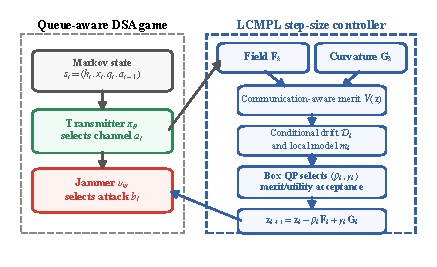
\includegraphics[width=0.98\columnwidth]{figures/algorithm_framework_queue.pdf}
\caption{LCMPL minimax policy-learning framework.}
\label{fig:framework}
\end{figure}

\section{Learning Stability and Communication Guarantees}
This section connects curvature-induced field-energy decrease to the implemented update and its finite-time communication guarantee.
Write $\nabla\bF=\bS+\bW$, where $\bS=(\nabla\bF+\nabla\bF^{\mathsf T})/2$ and $\bW=(\nabla\bF-\nabla\bF^{\mathsf T})/2$.

\begin{proposition}[Curvature identity for adversarial policy learning]
\label{prop:curvature}
At every point where $\bF$ is differentiable, the Jacobian--field direction satisfies
\begin{equation}
\langle\nabla\phi,\bG\rangle=\norm{\bS\bF}^2-\norm{\bW\bF}^2.
\label{eq:skew_identity}
\end{equation}
Hence, $+\bG$ decreases the field energy when $\norm{\bW\bF}>\norm{\bS\bF}$.
\end{proposition}

The proof is given in Appendix~\ref{app:proof-curvature}.

Proposition~\ref{prop:curvature} explains why the curvature coordinate can reduce field energy.
In particular, antisymmetric coupling creates the rotation of the field step and the inward action of the Jacobian--field correction.
The next conditions connect that ideal geometry to the local model and accepted learning update.
Define $D_F(\bz)=\langle\nabla V(\bz),\bF(\bz)\rangle$ and $D_G(\bz)=-\langle\nabla V(\bz),\bG(\bz)\rangle$, the first-order decreases of $V$ along $-\bF$ and $+\bG$.
Write $\Delta V_k=V(\bz_{k+1})-V(\bz_k)$.
\begin{assumption}[Local regularity and model accuracy]
\label{ass:model}
\begin{enumerate}
\item[(a)] A compact set $\mathcal T$ contains the accepted iterates and candidate segments, and $\bF\in C^1$ and $V\in C^2$ on a neighborhood of $\mathcal T$.
\item[(b)] For a fixed $s>0$, both pure-coordinate pairs $s\boldsymbol e_1$ and $s\boldsymbol e_2$ belong to $\mathcal U_k$, where $\boldsymbol e_i$ is the $i$th coordinate vector.
\item[(c)] Finite nonnegative $\mathcal F_k$-measurable errors $\epsilon_k^{\rm acc}$ and $\epsilon_k^{\rm mdl}$ satisfy
\[
\begin{aligned}
\E[\Delta V_k\mid\mathcal F_k]
&\leq \E[m_k(\widetilde{\bu}_k)\mid\mathcal F_k]+\epsilon_k^{\rm acc},\\
\E[m_k(s\boldsymbol e_i)\mid\mathcal F_k]
&\leq-sD_i(\bz_k)+\epsilon_k^{\rm mdl},\quad i\in\{1,2\},
\end{aligned}
\]
where $D_1=D_F$ and $D_2=D_G$.
\end{enumerate}
\end{assumption}
These errors aggregate policy-gradient and Jacobian-action noise, the directional-model approximation, and the acceptance step.
For the exact finite-game updates reported here, they record local-model and acceptance mismatch; sampled implementations additionally contribute estimation error.

Define the field-energy decrease signals
\[
\chi_F(\bz)=\bF^{\mathsf T}\bS\bF,
\quad
\chi_G(\bz)=-\langle\nabla\phi(\bz),\bG(\bz)\rangle.
\]
Positive $\chi_F$ and $\chi_G$ certify decrease of $\phi$ along $-\bF$ and $+\bG$, respectively.
\begin{assumption}[Geometric coverage]
\label{ass:geometry}
The local coverage modulus
\begin{equation}
m_{\rm geo}
=\inf_{\substack{\bz\in\mathcal T\\\norm{\bF(\bz)}>0}}
\frac{\max\{\chi_F(\bz),\chi_G(\bz)\}}{\norm{\bF(\bz)}^2}
\label{eq:coverage}
\end{equation}
satisfies $m_{\rm geo}>0$.
\end{assumption}
Geometric coverage holds when either the field or curvature coordinate decreases field energy at a rate proportional to $\|\bF\|^2$, allowing rotational points where the field coordinate is not a strict descent direction.
Let $\sigma_{\min}$ denote the smallest singular value.
At a target stationary point $\bz^\star$, the conditions $\bS(\bz^\star)\succeq0$ and $\sigma_{\min}(\nabla\bF(\bz^\star))>0$ imply Eq.~\eqref{eq:coverage} on a sufficiently small neighborhood by compactness of the unit sphere and continuity; this includes nonsingular pure rotation, where $\chi_F=0$ and $\chi_G>0$.
Compactness and smoothness make
\[
B_{\rm c}=\sup_{\bz\in\mathcal T}
\max\{\lvert\langle\nabla\mathcal L_{\rm c},\bF\rangle\rvert,
\lvert\langle\nabla\mathcal L_{\rm c},\bG\rangle\rvert\}<\infty.
\]
Because $V=\phi/\phi_0+\mathcal L_{\rm c}$, the larger of the field and curvature directional signals satisfies
\begin{equation}
\begin{aligned}
\max\{D_F(\bz),D_G(\bz)\}
&\geq\mu_{\rm geo}\norm{\bF(\bz)}^2-B_{\rm c},\\
\mu_{\rm geo}&=m_{\rm geo}/\phi_0.
\end{aligned}
\label{eq:geometry_certificate}
\end{equation}

Define the total conditional learning residual
\begin{equation}
\mathcal E_k(s)=sB_{\rm c}+\epsilon_k^{\rm acc}+\epsilon_k^{\rm mdl}.
\label{eq:residual}
\end{equation}
This single term separates the geometric benefit of the bi-direction update from stochastic sampling, local approximation, and acceptance errors.

\begin{figure*}[t]
\centering
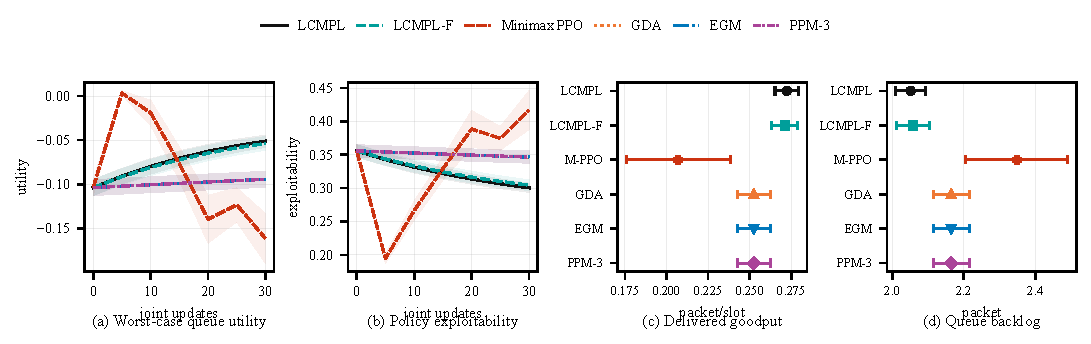
\includegraphics[width=\widefigwidth]{results/queue_nominal_benchmark.pdf}
\caption{Queue-aware nominal benchmark at moderate load over 12 seeds. Curves show means with one standard error; points show final means with 95\% confidence intervals.}
\label{fig:queue_nominal}
\end{figure*}

\begin{proposition}[Conditional Lyapunov drift]
\label{prop:drift}
Under Assumptions~\ref{ass:model}--\ref{ass:geometry}, the accepted update satisfies
\[
\begin{aligned}
&\E[V(\bz_{k+1})-V(\bz_k)\mid\mathcal F_k]\\
&\leq-s\mu_{\rm geo}\norm{\bF(\bz_k)}^2
+\mathcal E_k(s).
\end{aligned}
\]
\end{proposition}

The proof is given in Appendix~\ref{app:proof-drift}.

\begin{theorem}[Main finite-time minimax stationarity result]
\label{thm:stationarity}
Under Assumptions~\ref{ass:model}--\ref{ass:geometry}, every integer $K\geq1$ satisfies
\begin{equation}
\frac1K\sum_{k=0}^{K-1}\E\norm{\bF(\bz_k)}^2
\leq
\frac{V(\bz_0)}{s\mu_{\rm geo}K}
+\frac{\overline{\mathcal E}_K(s)}{s\mu_{\rm geo}},
\label{eq:rate}
\end{equation}
where $\overline{\mathcal E}_K(s)=K^{-1}\sum_{k=0}^{K-1}\E\mathcal E_k(s)$.
\end{theorem}

The proof is given in Appendix~\ref{app:proof-theorem}.

If $\sup_k\E\mathcal E_k(s)\leq\bar E<\infty$, Theorem~\ref{thm:stationarity} gives an $O(1/K)$ transient plus the floor $\bar E/(s\mu_{\rm geo})$.
It covers pure rotation: the field has zero first-order effect, while curvature supplies the strict decrease in Fig.~\ref{fig:motivation} and Proposition~\ref{prop:curvature}.
Here, $s$ serves as an analytical comparator, whereas $\beta_k$ and $\gamma_k$ are the implemented step sizes.

The following local compatibility condition bridges Theorem~\ref{thm:stationarity} from neural parameter-space stationarity to full-policy best responses.

Let $v^*=\max_{\pi\in\Pi_{\rm T}}\min_{\nu\in\Pi_{\rm J}}J(\pi,\nu)$ denote the unregularized stationary-policy game value.
Since each $M$-ary policy has entropy at most $\log M$, the regularized and unregularized returns differ by at most $\tau\log M$ for either player.
Consequently,
\begin{equation}
0\leq v^*-U_{\rm BR}(\btheta)\leq\Delta_\tau(\bz)+2\tau\log M.
\label{eq:performance_bridge}
\end{equation}
Let $B_K$ denote the right-hand side of Eq.~\eqref{eq:rate}.

\begin{corollary}[Main communication result: worst-case utility]
\label{cor:rate}
If nonnegative constants $C_{\rm gap}$ and $\xi_{\rm gap}$ satisfy $\Delta_\tau(\bz)\leq C_{\rm gap}\norm{\bF(\bz)}^2+\xi_{\rm gap}$ on $\mathcal T$, then
\[
\frac1K\sum_{k=0}^{K-1}\E\big[v^*-U_{\rm BR}(\btheta_k)\big]
\leq C_{\rm gap}B_K+\xi_{\rm gap}+2\tau\log M.
\]
\end{corollary}

The proof is given in Appendix~\ref{app:proof-corollary}.

The last term is the entropy-regularization error.

\begin{figure*}[t]
\centering
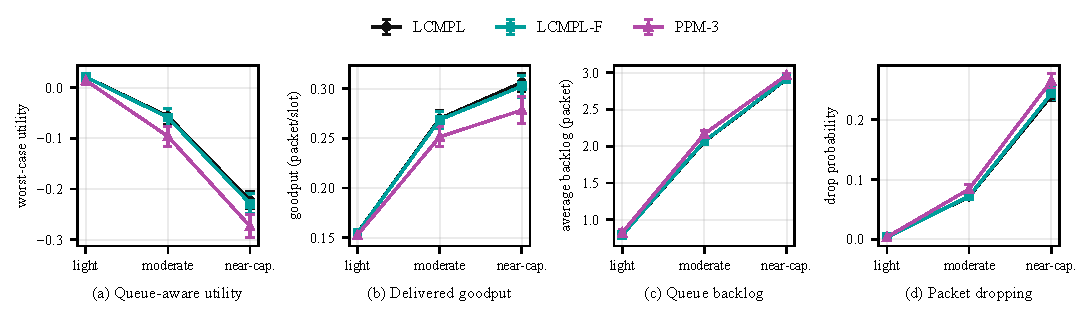
\includegraphics[width=\widefigwidth]{results/queue_load_results.pdf}
\caption{Traffic-load stress over 12 seeds. Error bars are 95\% confidence intervals; light, moderate, and near-capacity loads use $\lambda_A=0.20$, $0.45$, and $0.70$.}
\label{fig:queue_load}
\end{figure*}

\section{Communication Performance Evaluation}
We evaluate worst-case discounted utility, exploitability, delivered goodput, backlog, and dropping in the action-dependent queueing game.
Both agents use independent one-hidden-layer tanh--softmax neural policies, so Fig.~\ref{fig:queue_nominal}(a)--(b) directly evaluate neural minimax-learning convergence.
Matched comparisons share the environment, policy architecture, initialization, seeds, entropy coefficient, and simultaneous start.
The nominal benchmark compares GDA~\cite{Mokhtari2020UnifiedEG}, the extragradient method (EGM)~\cite{Korpelevich1976Extragradient}, PPM-3 as three inner fixed-point iterations approximating the proximal point method (PPM)~\cite{Rockafellar1976PPM}, clipped minimax proximal policy optimization (Minimax PPO)~\cite{Schulman2017PPO}, LCMPL-F with $\gamma_k=0$, and LCMPL.
Appendix~\ref{app:reproducibility} reports the complete protocol.

\subsection{Neural Learning Dynamics and Policy Quality}
The nominal study asks whether curvature selection improves both the training dynamics and the communication quality of the learned neural policies under moderate traffic.
Fig.~\ref{fig:queue_nominal}(a)--(b) show the convergence of worst-case utility and exploitability over 30 joint neural-policy updates, while Fig.~\ref{fig:queue_nominal}(c)--(d) report final goodput and backlog.
LCMPL simultaneously raises worst-case utility and reduces exploitability.
Relative to LCMPL-F, its paired mean utility gain is $0.0024$ (95\% confidence interval $[0.0001,0.0047]$), while exploitability decreases by $0.0039$ ($[0.0007,0.0071]$).
The same accepted policies increase delivered goodput by $0.0012$ packet/slot ($[0.0001,0.0024]$) and reduce backlog by $0.0066$ packet ($[0.0006,0.0126]$).
Against GDA, EGM, and PPM-3, LCMPL gains about $0.0431$ in utility and $0.0198$ packet/slot in goodput while reducing backlog by $0.1138$ packet; every paired 95\% interval excludes zero.
Fig.~\ref{fig:queue_nominal}(c) and Fig.~\ref{fig:queue_nominal}(d) therefore connect saddle stabilization to packet delivery rather than only to an optimization residual.

\subsection{Load-Adaptive Communication Robustness}
The second study tests whether the value of selective curvature grows as endogenous queueing stress tightens the service margin.
Fig.~\ref{fig:queue_load} varies only the arrival rate from light through moderate to near-capacity traffic while retaining the same radio model, neural architecture, seeds, and evaluation rule.
At light load, LCMPL and LCMPL-F are statistically indistinguishable because service is sufficient and the controller seldom needs curvature.
The fraction of LCMPL updates with $\gamma_k>10^{-10}$ rises from $8\%$ to $44\%$ and $71\%$ across the three loads.
At moderate and near-capacity loads, the utility gains over LCMPL-F are $0.0023$ and $0.0064$, respectively, with positive paired 95\% confidence intervals.
Near capacity, LCMPL also increases goodput by $0.0037$ packet/slot and reduces backlog and drop probability by $0.0061$ packet and $0.0034$, respectively.
The increasing gain shows why local selection matters: suppressing rotational updates has little effect when the queue drains easily but prevents learning oscillations from accumulating into congestion under tight service margins.

\section{Conclusion}
LCMPL separates field and curvature step sizes in queue-aware adversarial DSA and retains curvature only when the acceptance test validates merit and physical utility.
The analysis bounds time-averaged stationarity and, under a local policy-gap condition, worst-case utility loss.
The experiments show that this geometric stabilization improves packet delivery and limits backlog precisely where adversarial learning errors are most costly: near the queue's service boundary.

\appendices
\section{Proofs}
\label{app:supplement}
\subsection{Proof of Proposition~\ref{prop:curvature}}
\label{app:proof-curvature}
With $\bA=\nabla\bF$, $\langle\nabla\phi,\bG\rangle=\bF^{\mathsf T}\bA^2\bF$.
Expanding $\bA=\bS+\bW$ and using antisymmetry of $\bS\bW+\bW\bS$ give Eq.~\eqref{eq:skew_identity} because $\bF^{\mathsf T}\bS^2\bF=\|\bS\bF\|^2$ and $\bF^{\mathsf T}\bW^2\bF=-\|\bW\bF\|^2$.
\hfill$\square$

\subsection{Proof of Proposition~\ref{prop:drift}}
\label{app:proof-drift}
The QP optimum is no larger than either comparator in Assumption~\ref{ass:model}(b); Assumption~\ref{ass:model}(c) and Eq.~\eqref{eq:geometry_certificate} transfer this dominance to the accepted Lyapunov change.
\hfill$\square$

\subsection{Proof of Theorem~\ref{thm:stationarity}}
\label{app:proof-theorem}
Take total expectations in Proposition~\ref{prop:drift}, sum over $k$, and use $V(\bz_K)\geq0$ to obtain Eq.~\eqref{eq:rate}.
\hfill$\square$

\subsection{Proof of Corollary~\ref{cor:rate}}
\label{app:proof-corollary}
Average Eq.~\eqref{eq:performance_bridge}, apply the local gap condition, and invoke Theorem~\ref{thm:stationarity}.
\hfill$\square$

\section{Reproducibility Details}
\label{app:reproducibility}
Both experiments use $M=L=4$, $Q_{\max}=4$, $\rho_h=0.75$, $R_0=1$, $N_0=1$, $I_t^{\rm pri}=0$, $g_t^J=1$, $P_{\rm s}=10$, $P_{\rm J}=18$, $c_{\rm sw}=0.05$, adjacent leakage $0.50$, $\delta=0.95$, and $\tau=0.02$.
The modes cyclically shift $g_m^{\rm base}$ geometrically from $1.9$ to $0.30$; nonadjacent leakage is $0.08$.
The utility weights are $(\alpha_q,\alpha_d)=(0.12,0.60)$.
Independent one-hidden-layer tanh--softmax policies observe $(g_t,q_t,a_{t-1})$, use 32 hidden units, and have 452 parameters per player.
The nominal benchmark uses $\lambda_A=0.45$, 30 updates, and all six methods; the load stress uses $\lambda_A\in\{0.20,0.45,0.70\}$, 25 updates, and LCMPL, LCMPL-F, and PPM-3.
Both use the 12 fixed seeds 600--611 with an initially empty queue and uniformly sampled $h_0$ and $a_{-1}$.
Fixed-step GDA, EGM, and PPM-3 use $0.01$; Minimax PPO uses $10^{-3}$.
LCMPL uses the box $[0,0.08]\times[0,0.12]$, weights $(\lambda_\Delta,\lambda_U)=(0.35,1.5)$, initial-value normalization, and the released directional-model and acceptance tolerances.

\bibliographystyle{IEEEtran}
\bibliography{refs}

\end{document}
